%
%  Chapter:  3 - 135Pr Experimental Methods
%  Modified: 2/16/2015
%  Author:   James Till Matta
%
%%%%%%%%%%%%%%%%%%%%%%%%%%%%%%%%%%%%%%%%%%%%%%%%%%%%%%%%%%

\chapter{EXPERIMENTAL METHODS}
\label{chp:exp-pr}
Across all of experimental physics there is a common theme in the design of an experiment. Finding a way of producing the system to be studied is one part of this theme. The other part is having the equipment to collect the signals necessary to understand what the system is doing. In nuclear physics, the appropriate choice of reaction will create the desired system and the equipment for signal collection will depend greatly on what one wishes to measure. This chapter will discuss the reaction, detectors, and techniques used in the examination of transverse wobbling in \pr{}.
\section{Heavy-ion Fusion-evaporation Reaction}
\label{sec:exp-pr-fus-evap}
Across nuclear physics there are vast array of reactions used. Narrowing to in-beam \gr{} spectroscopy one finds some common ``workhorse'' reactions that are commonly used. Of these workhorse reactions the heavy-ion fusion-evaporation reaction is frequently chosen for its selectivity in final products, producing relatively few species with large cross-section, and its creation of states with a large amount of angular momentum.\cite{beausang1996arrays}.
\subsection{Creation and Decay of the Compound Nucleus}
\label{ssec:exp-pr-fus-evap-cn}
The fusion evaporation reaction proceeds by the formation of a highly excited compound nucleus, a mechanism first proposed by Neils Bohr\cite{bohr1936neutron}. While it is possible for a compound nucleus to be formed for beam energies below the coulomb barrier the probability is dramatically lower as the beam must quantum mechanically tunnel through same barrier. Therefor for heavy ion fusion to be experimentally feasible the center of momentum energy must exceed the height of the coulomb barrier. The coulomb barrier height can be estimated with

\begin{equation}
\label{eqn:cb_en}
E_{CB}=\frac{\alpha \hbar c Z_p Z_t}{1.16 fm (A_p^{1/3} + A_t^{1/3} + 2)}
\end{equation}

and the non-relativistic center of momentum energy is

\begin{equation}
\label{eqn:cmf_en}
E_{cm} = \frac{\mu}{A_{p}}E_{p}
\end{equation}

Here the subscripts $p$ and $t$ denote projectile and target respectively, $A$ is the mass number, $Z$ represents the nuclear charge, $\alpha{}$ is the fine structure constant, and $\mu = A_{p}A_{t}/(A_{p}+A_{t})$ is the system's reduced mass. After its formation the compound nucleus will have an excitation energy of

\begin{equation}
\label{eqn:cn_ex}
E_{ex} = Q + E_{cm}
\end{equation}

where $Q$ is the reaction's $Q$-value which is,

\begin{equation}
\label{eqn:cn_form_qvalue}
Q = (M_t+M_p-M_{CN})c^2
\end{equation}

The compound nucleus will also carry an angular momentum ranging between $0 \hbar$ and $l_{max} \hbar$, corresponding to head on and peripheral collisions respectively. $l_{max}$ can be estimated classically as

\begin{equation}
\label{eqn:cn_lmax}
l_{max} = \frac{\sqrt{2\mu(E_{cm}-E_{CB})}}{4}(A^{1/3}_p + A^{1/3}_t)\hbar
\end{equation}

Following its formation a compound nucleus will be left in a state of high excitation energy. The two primary ways the compound nucleus rids itself of this excess energy are fission or particle evaporation followed by \gr{} emission. A schematic of of a fusion evaporation reaction can be found in Fig. \ref{fig:chp3-fus-evap-schem}.

\begin{figure}[h!]
	\centerline{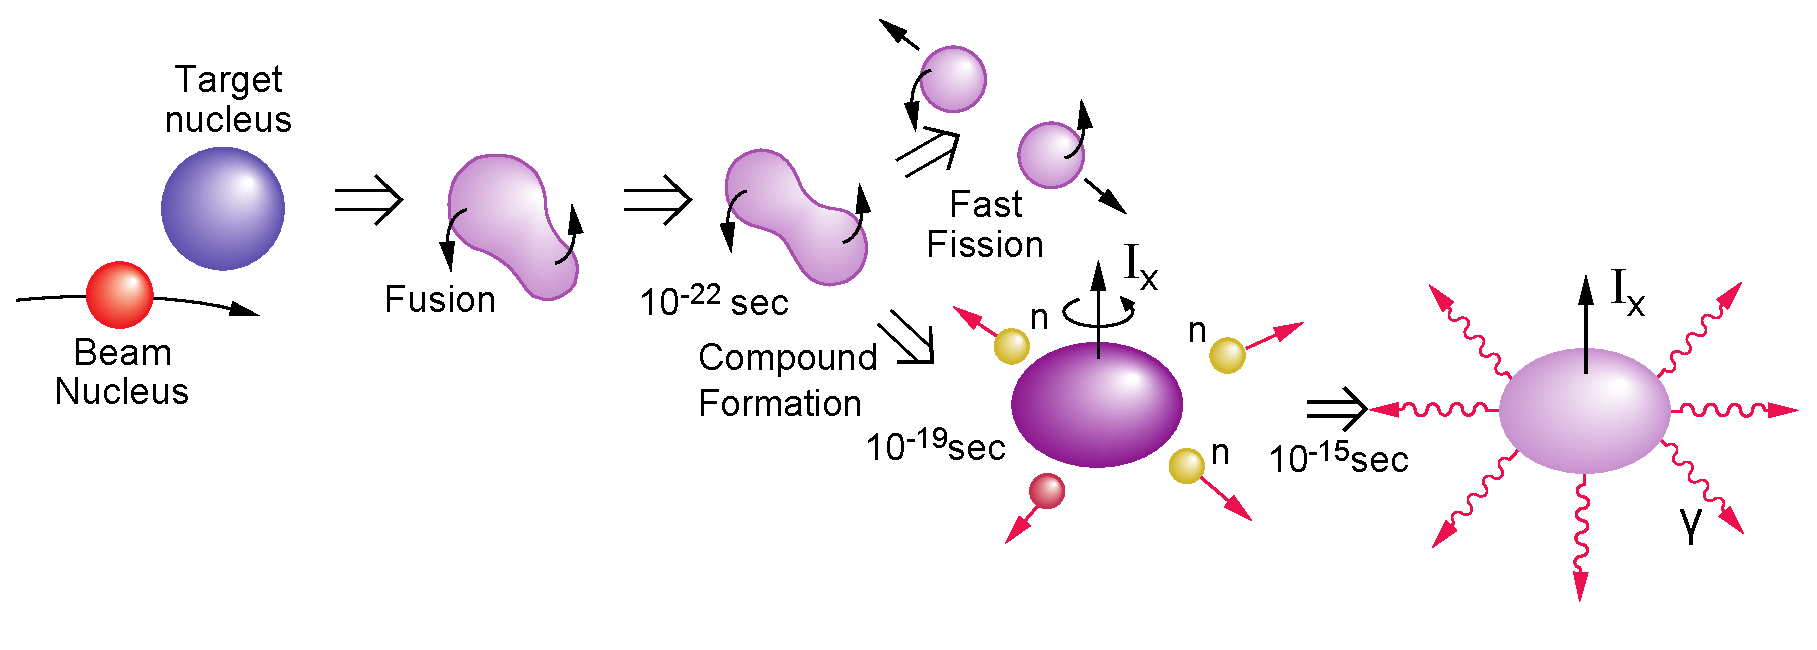
\includegraphics[width=\textwidth]{./img/c3/fusion_evaporation.pdf}}
	\caption{Schematic illustration of heavy-ion fusion-evaporation, adapted from Ref. \cite{gsBooklet}.}
	\label{fig:chp3-fus-evap-schem}
\end{figure}

The probability of the compound nucleus fissioning is governed by the height of the fission barrier relative to the its excitation energy. The height of the fission barrier is a function of the $A$ of the nucleus and is inversely proportional to the compound nucleus' angular momentum, as can be seen in Fig. \ref{fig:chp3-fission-barrier}. It should be noted, that even the complete disappearance of the fission barrier does not guarantee fission as there are, a few, observed cases of spins above those required to reduce the barrier to zero\cite{hyperdef,hyperdef2}.

\begin{figure}[h!]
	\centerline{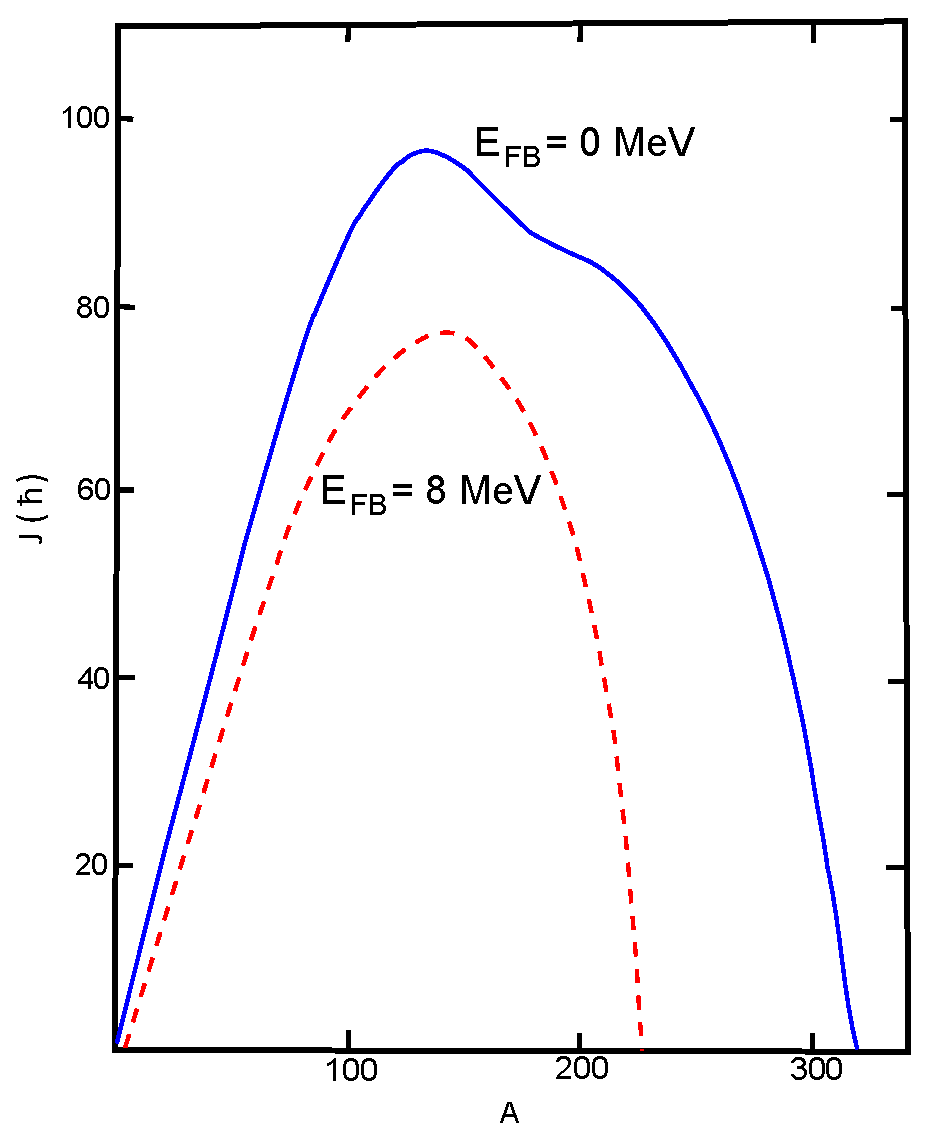
\includegraphics[height=0.3\textheight]{./img/c3/fission_barrier.eps}}
	\caption{Isocontours of angular momenta that yield fission barriers of $8MeV$ and $0MeV$ at various masses. Adapted from Ref. \cite{fissionBarrier2}.}
	\label{fig:chp3-fission-barrier}
\end{figure}

If the compound nucleus does not fission then it will instead evaporate particles. Particle evaporation is the emission of protons, neutrons, or alpha particles over or through an emission barrier. For charged particles this emission barrier is composed both of a centrifugal term which grows with increasing angular momentum and a coulomb term. For neutrons the emission barrier is solely the centrifugal barrier. As charged particles see a higher barrier due to the coulomb term, neutron evaporation is more probable in most cases. The exception occurs for very neutron deficient nuclei where the reduced proton separation energies make it possible for charged particle emission to compete with, or even dominate charged particle emission. Each successive evaporated particle carries energy, but little angular momentum away from the nucleus until there is insufficient excitation energy for particles to penetrate the emission barrier and the nucleus is left in a state that is stable against particle emission. From this point on the nucleus must dissipate its excess angular momentum and excitation energy via \gr{} emission. A schematic of this can be seen in Fig. \ref{fig:chp3-emission-schematic}.

\begin{figure}[h!]
	\centerline{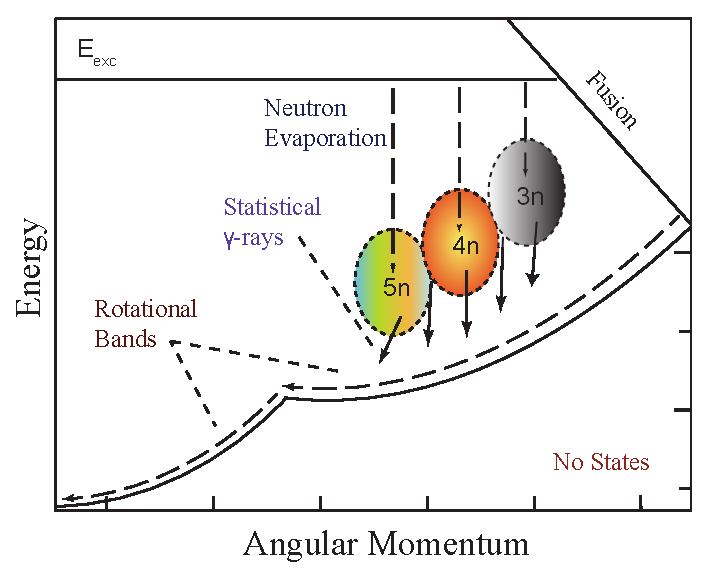
\includegraphics[height=0.3\textheight]{./img/c3/evaporation_chans.eps}}
	\caption{Schematic of the compound nuclear decay assuming that a rotational nucleus is being formed. Adapted from Ref. \cite{danielDissertation}.}
	\label{fig:chp3-emission-schematic}
\end{figure}

Initially the nucleus is in a state with such high level density that it decays by the emission of statistical \gr{}s\cite{cnCooling}. These statistical \gr{}s are almost purely dipole in nature and form a continuum as the notion of a discrete state is not a good one at such high level densities. As the nucleus approaches the yrast line (the states with the minimum excitation energy for a given angular momentum) the level density drops. This allows the emission sequences of discrete \gr{}s which feed the yrast line.

\subsection{Choice of Beam and Target}
\label{ssec:exp-pr-fus-evap-beam-target}
When choosing the beam and target for a fusion evaporation one must consider several factors: What is the production cross-section of the desired residual nucleus? How clean is the production of the desired residual nucleus relative to the other residuals? What is the spin range one wishes to study? What is the availability of the isotopes desired? What is the suitability of the material for beam production? While beam target combinations are usually chosen to maximize the cross-section for the desired residual, in some cases there are other channels open which will have large cross-sections themselves. In these cases the beam-target combination might be chosen to drastically lower the relative yield in competing channels at the cost of lowering the cross-section for the desired residual. For lower spins one usually chooses lighter projectiles. While Eqn. \ref{eqn:cn_lmax} clearly shows that it is possible to increase the angular momentum transfer with higher beam energies, this also increases the excitation energy of the compound nucleus, causing particle evaporation to be more probable. In the end, the decision is based on what combination yields the nucleus one wishes to study in the spins one wishes to study with the highest absolute and relative cross-sections possible.

Ref \cite{nucSpecAndReacPartC} gives the empirical estimate for $A_{CN}>100$ for obtaining the optimum beam energy for producing a specific residual nucleus in a (HI,xn) reaction which can be found in Eqn. \ref{eqn:fe_peak_selection}.
\begin{equation}
\label{eqn:fe_peak_selection}
E_{pk}(x)=(-Q_{x} + \alpha{}x)(1+\frac{A_p}{A_t})
\end{equation}
Here $Q_x$ is the Q-value for the production of the residual nucleus given by:
\begin{equation}
\label{eqn:res_qvalue}
Q = (M_t+M_p-M_{res}-x M_n)c^2
\end{equation}
and $\alpha$ is $\sim6MeV$. Of course, the reaction will only have a reasonable cross-section if $E_{pk}(x)$ is greater than $E_{CB}$, which is the height of the coulomb barrier, given in Eqn. \ref{eqn:cb_en}. In more modern times computer codes that employ statistical models such as PACE4\cite{PACE4,PACE4_2} can be used to calculate the cross-sections of products from these reactions allowing one to estimate peak beam energies and optimal beam-target combinations. A plot of cross-sections yielded by calculations such as these can be found in Fig. \ref{fig:chp3-pace4-calc}

\begin{figure}[h!]
	\centerline{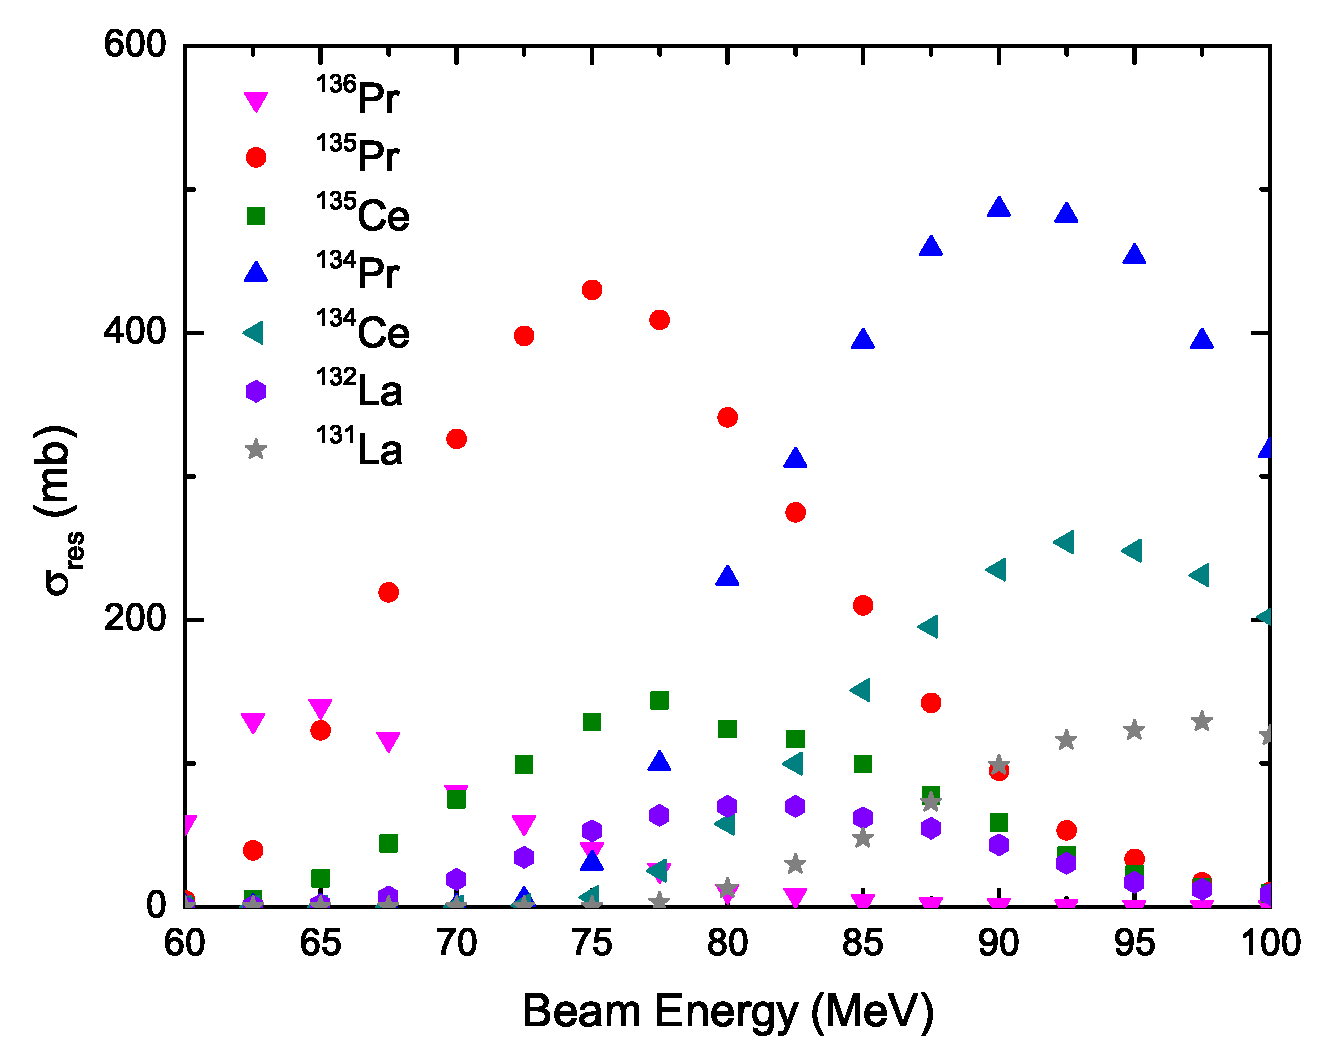
\includegraphics[width=\textwidth]{./img/c3/135Pr_calc_plot.eps}}
	\caption{Cross-sections of various residual nuclei for a $^{16}$O beam on $^{123}$Sb at a variety of beam energies as calculated by PACE4. As $^{139}$Pr is the compound nucleus produced all products that are not isotopes of Pr require the evaporation of a charged particle.}
	\label{fig:chp3-pace4-calc}
\end{figure}

\section{Gamma-ray Spectroscopy}
\label{sec:exp-pr-gamma-spec}
\subsection{Gamma-ray Interaction with Matter}
\label{ssec:exp-pr-gamma-spec-interactions}
As mentioned earlier, the choice of equipment will vary with which signals you need to collect to understand the system. In the case of a residual nucleus at high spin one of the obvious signal choices is the \gr{}s it emits. Detection of gamma-rays is dependent on the \gr{} depositing energy in a detector which in turn depends on the interactions of electromagnetic radiation with matter. At the energies relevant to nuclear physics, $10keV<E_{\gamma}<15MeV$, there are three primary processes to be considered, photoelectric absorption, Compton scattering, and pair production. These three processes compete with each dominating in a different energy range.

In photoelectric absorption the photon interacts with a bound electron in the detector material and is fully absorbed\cite{einstein-PE}. The total energy of the photon is then used to overcome the binding energy of the electron and to provide the electron with kinetic energy, giving $E_{e^-}=E_{\gamma}-E_b$. The electron then proceeds to lose energy as it passes through the detector material. In \gr{} spectra the full energy peak corresponds to the deposition of the photon's full energy in the detector medium. For that to occur either the primary photon, or all the secondary photons (generated by the processes below), must undergo photoelectric absorption. As can be seen in Fig. \ref{fig:chp3-gamma-interactions} the photoelectric effect is dominant at low energies and the energy at which the photoelectric effect ceases to dominate increases with the Z of the material.

\begin{figure}[h!]
	\centerline{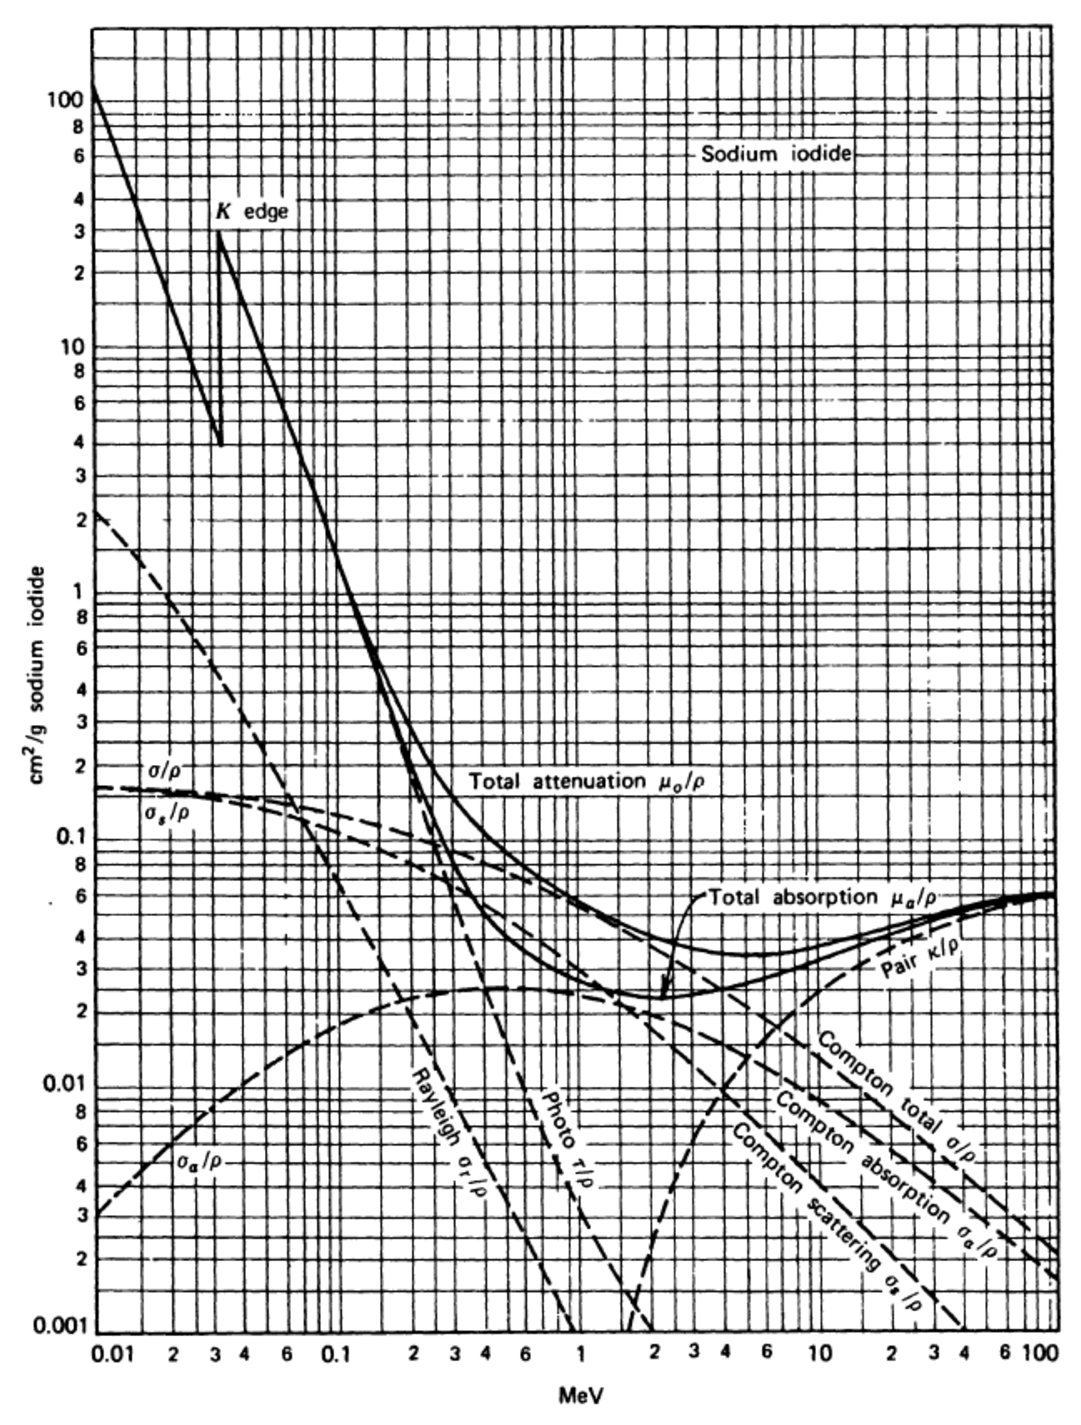
\includegraphics[height=0.5\textheight]{./img/c3/gamma_interactions_scan.eps}}
	\caption{Gamma-ray attenuation coefficients for various processes in NaI, adapted from Ref. \cite{knollBook}. Here we can see the dominance of photoelectric absorption at lower energies, Compton scattering at intermediate energies and pair production at high energies. While the slopes of these processes changes from material to material the trends remain the same.}
	\label{fig:chp3-gamma-interactions}
\end{figure}

In Compton scattering, a \gr{} photon scatters from an electron in the material at some angle $\theta$ to its original direction\cite{Compton-PhysRev.21.483}. Due to conservation of momentum and energy, the energy transferred to the electron is precisely determined by $\theta$ and so the energy of the secondary photon can be written as: $E_{s}=E_{p}(1+\frac{E_{p}}{m_{e}c^2}(1-Cos\theta))^{-1}$ As above the electron then deposits its kinetic energy in the medium as it slows. However, unlike in the photoelectric effect, not all of the energy is deposited in the electron. After the scattering the secondary photon travels in its new direction and is free to interact again with probabilities dictated by its energy. As shown in Fig. \ref{fig:chp3-gamma-interactions} Compton scattering is the dominant effect at intermediate energies.

The final process to be considered is pair production. In pair production the photon enters the region of very strong electric field near the nucleus and its energy is converted into the mass and kinetic energy of an electron positron pair \cite{anderson-PhysRev.43.491,oppenheimer_PhysRev.44.53.2}. Since energy is conserved the photon must have energy of at least twice the rest mass of the electron, giving a threshold of $E_{\gamma}\geq1.022MeV$ for this interaction, any energy above this threshold is converted into kinetic energy shared between the two particles. After their production the electron and positron will both travel through the detector medium loosing energy as they travel. Once at rest the positron will annihilate with an electron, emitting two anti-parallel $511keV$ secondary photons. Fig. \ref{fig:chp3-gamma-interactions} shows the dominance of this interaction at high gamma energies, the energy at which pair production supersedes Compton scattering decreases with increasing Z of the material.

\subsection{High Purity Germanium (HPGe) Detectors}
\label{ssec:exp-pr-gamma-spec-hpge}
In detecting gamma-rays there are essentially 3 major classes of detector, scintillator, gas, and semiconductor detectors. In all cases the \gr{} enters the active volume of the detector and deposits energy by at least one of the processes mentioned above, the primary energetic electrons, produced directly by the interactions of the \gr{}, then proceed to ionize or excite other electrons in the material, the secondary electrons are then detected in some manner. In scintillators they cause UV or visible light to be emitted and that is collected via photomultiplier or similar to produce a voltage pulse. In gas and semiconductor detectors the charge of the secondary electrons (and their corresponding ions or holes) is collected directly, albeit via different mechanisms, to produce the voltage pulse.

It is desirable that \gr{} detectors have both good detection efficiency and energy resolution. Unfortunately, in the \gr{} detectors presently available there is a conflict between these goals and so one must decide which parameter is more important. For high spin experiments where the spectrum is dense with peaks the energy resolution is the top priority as broad peaks would be indistinguishable from each other. Amongst the available detectors, semiconductor detectors, particularly High Purity Germanium (HPGe) detectors offer the best energy resolution.

Semiconductor detectors are reversed bias diodes with either a p-n or a p-i-n junction. At the boundary between the types of materials there is a so called contact potential. This potential gives rise to an electric field which causes the migration of charges between the two materials until there is an area bridging the boundary called the depletion zone. In this zone there is an electric field which gives rise to a potential that counters the contact potential. By applying reverse bias to the diode the contact potential is effectively increased causing the depletion zone to expand (schematic in Fig. \ref{fig:chp3-pn_diode}.) This is desirable because the depletion zone(s) are the only regions of the semiconductor where an electric field will exist. This means that electron hole pairs formed in the within it are swept away from each other before they can recombine so that they can be collected. In contrast, electron hole pairs formed outside the depletion zone are not pulled away from each other and recombine, preventing their collection. Due to this, the depletion zone of the detector is the region that is active. That is to say that the passage of ionizing radiation through the that region is detectable as electron hole pairs it produces will be collected.

\begin{figure}[h!]
	\centerline{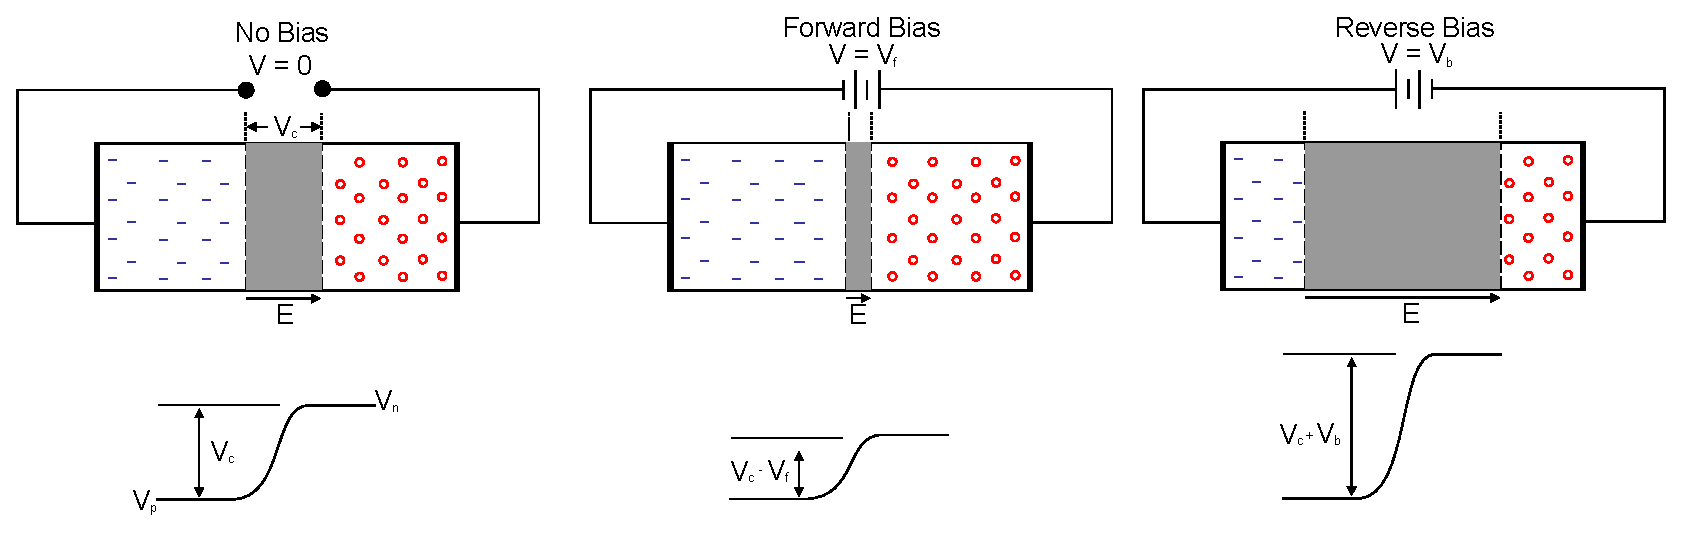
\includegraphics[width=\textwidth]{./img/c3/pn-diode.eps}}
	\caption{Above: Diagramatic view of the depletion zone's with varying bias voltage. Below: Voltage difference across the depletion zone for each bias voltage shown above}
	\label{fig:chp3-pn_diode}
\end{figure}

The higher the purity of the semiconductor, the higher the reverse bias voltage that can be applied without reaching the breakdown of the semiconductor (usually catastrophic event.) In HPGe detectors the purity is sufficiently high that the whole crystal of Ge can be depleted yielding a very large active region, an advantage for \gr{}s given their low interaction probabilities compared to charged particles. When a gamma interacts in an HPGe detectors it produces at least one high energy secondary electron or positron (more if there are multiple interactions). These secondary electrons lose energy quickly as they pass through the detector, leaving a trail of electron hole pairs in their wake. The electrons and holes are then swept to their respective contacts by the applied potential and collected.

A detectors resolution is defined the FWHM for a given peak. The intrinsic resolution of a semiconductor detector stems from statistical fluctuations in how many electrons and holes are collected at the terminals. As these fluctuations arise from simple counting statistics one their form can be deduced to be:
\begin{equation}
\label{eqn:hpge-res-est} 
\Delta{}E_{in} \propto \frac{E_{\gamma}}{\sqrt{N}}
\end{equation}
Where N is the number of charge carriers produced and is approximately $E_{\gamma}/\epsilon$ where $\epsilon$ is the average energy to make an electron hole pair ($2.96eV$ for Ge). In a more careful examination we see that the intrinsic component of the FWHM is:
\begin{equation}
\label{eqn:hpge-in-res} 
\begin{split}
\Delta{}E_{in}(E) & = 2\sqrt{2 ln(2)}\frac{\sqrt{F E_{\gamma{}}/\epsilon{}}}{E_{\gamma{}}/\epsilon{}}E_{\gamma{}}\\
       & = 2.355\sqrt{F\epsilon{}E_{\gamma{}}}
\end{split}
\end{equation}
Here $F$ is the Fano factor. This value, intrinsic to the detector material, ranges across $(0,1]$ and takes into account energy loss mechanisms available to the secondary electron(s) that do not generate electron hole pairs. The inquiring reader can find a more thorough explanation in Refs. \cite{knollBook,fano_factor1}.

Unfortunately, the detector's intrinsic resolution is not the only contributor to the detector's resolution. There are also contributions from such sources as electronic noise, charge carrier collection / trapping, and Doppler broadening. If one assumes that these components are independent and normally distributed one gets the actual resolution to be:
\begin{equation}
\label{eqn:hpge-res} 
\Delta{}E_{T}^2 = \Delta{}E_{in}^2 + \Delta{}E_{E}^2 + \Delta{}E_{C/T}^2 + \Delta{}E_{D}^2
\end{equation}
Where $\Delta{}E_{E}$ is the electronic noise contribution, $\Delta{}E_{C/T}$ is the charge collection / trapping term, and $\Delta{}E_{D}$ is the Doppler broadening term. Ref. \cite{trappingResolution} gives the FWHM forms of the noise and collection / trapping terms to be:
\begin{equation}
\label{eqn:hpge-res-noise} 
\Delta{}E_{E} = N_{1/2}
\end{equation}
\begin{equation}
\label{eqn:hpge-res-ct} 
\Delta{}E_{C/T} = 2.355\sqrt{\epsilon{} K E_{\gamma{}} [1-\eta{}(r)]}
\end{equation}
Where $N_{1/2}$ is the FWHM of the electronic noise, $K$ is a constant of a given detector, and $\eta{}(r)$ is the total charge collection efficiency of electrons and holes of the detector as a function of the interaction site's radius.

\begin{figure}
	\centerline{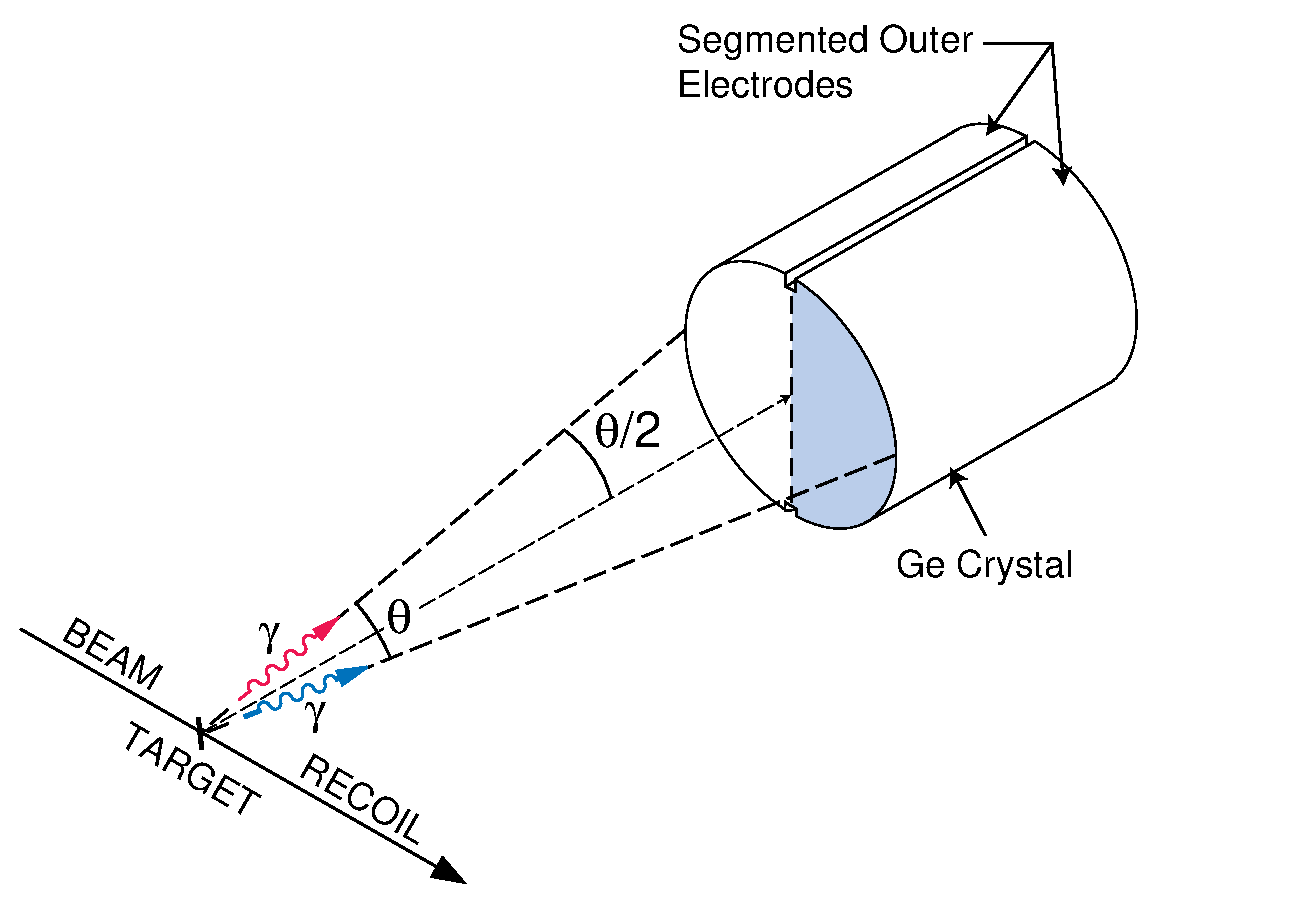
\includegraphics[height=0.3\textheight]{./img/c3/split_contact.eps}}
	\caption{Diagram showing the uncertainty inherent in the \gr{}'s angle of emission, as well as Gammasphere's segmented electrode scheme to reduce this.}
	\label{fig:chp3-doppler-split-contact}
\end{figure}

The final term, $\Delta{}E_{D}$, of this equation comes from uncertainty in the angle at which the gamma ray was emitted from the recoiling nucleus due to the detectors finite size (shown in Fig. \ref{fig:chp3-doppler-split-contact}.) The shift in gamma energy due to the nuclear recoil is:
\begin{equation}
\label{eqn:doppler_formula} 
E_{o} = E_{e}\frac{\sqrt{1+\beta{}Cos(\theta)}}{\sqrt{1-\beta{}Cos(\theta)}}
\end{equation}
here, the subscripts o and e refer to observed and emitted, $\beta$ is the speed of the recoiling nucleus and theta is the angle between the nucleus' line of a flight and the emitted \gr{}. If the detector has an angular acceptance such that $\theta{}_{0}-\delta{}\theta{}\leq{}\theta{}\leq{}\theta{}_{0}+\delta{}\theta{}$ with $\theta{}_{0}$ the central angle of the detector; we find that, to first order, the contribution of Doppler broadening is:
\begin{equation}
\label{eqn:res-doppler-term} 
\Delta{}E_{D} = 2\beta{}Sin(\theta{})Sin(\delta{}\theta{})E_{\gamma}
\end{equation}
There are three strategies to combat this term. The first is geometrical. By increasing the granularity of the array, either by using more, smaller detectors, or by using more detectors at a longer distance from the source. This in turn would shrink the opening angle of detectors and therefor reduce the Doppler broadening. The second method is electrical in nature, by segmenting the outer contact of the detector, even roughly, one can localize within the detector where the interaction occurred, therefor effectively reducing the opening angle. Gammasphere uses this strategy as shown in Fig. \ref{fig:chp3-doppler-split-contact}. The split outer contact lets one reduce the effective opening angle, $2\delta{}\theta{}$, from $14.9^{\circ}$ to $7.45^{\circ}$ \cite{TheGS}. The third method involves a physical segmentation of the detector, by having multiple crystals in close proximity within the same cryostat. This, give a detector that has a volume equal to the sum of the individual crystal volumes.However the opening angle of the individual crystals is the opening angle to consider for the Doppler broadening. Thus a physically segmented detector can give you a smaller Doppler broadening than an unsegmented detector of the same volume.  Clover and cluster detectors\cite{cloverDet,clusterDetector} are examples of this strategy.

\subsection{Escape Suppression with BGO detectors}
\label{ssec:exp-pr-gamma-spec-escape-supress}
The primary contribution to the background in \gr{} spec is the incomplete deposition of energy in the detector. Two of the mechanisms discussed in section \ref{ssec:exp-pr-gamma-spec-interactions} can lead to this. Compton scattering will result in incomplete energy deposition when the secondary photon yielded by the process may escape the HPGe crystal without depositing the rest of its energy. This mode results in a smooth background from the maximum energy transferable to an electron in the process down to zero energy. Pair production will yield incomplete energy deposition when one or both of the photons from the annihilation of the positron escape the detector. This mode results in 2 new peaks forming, the first $511keV$ below the photopeak, corresponding to one annihilation photon escaping, and a second $1022keV$ below the photopeak, corresponding to both escaping.
\begin{figure}[h!]
	\centerline{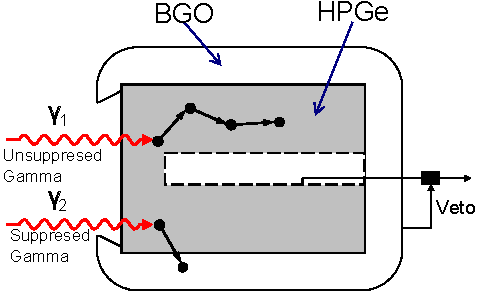
\includegraphics[height=0.25\textheight]{./img/c3/BGO_schematic.pdf}}
	\caption{Schematic of BGO escape suppression around an HPGE crystal.}
	\label{fig:chp3-supression-schematic}
\end{figure}
\begin{figure}[h!]
	\centerline{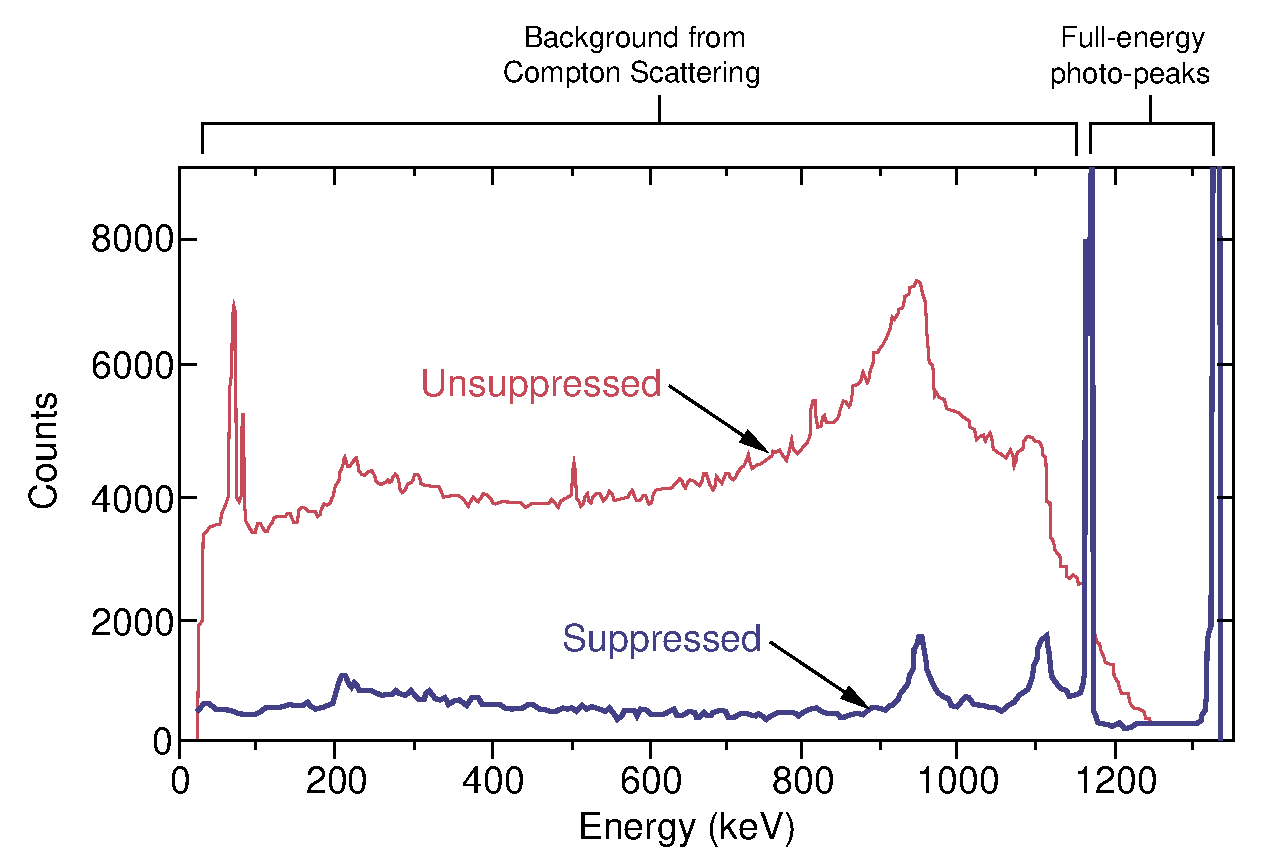
\includegraphics[height=0.25\textheight]{./img/c3/suppressed_spectra.eps}}
	\caption{Superimposed spectra of an escape suppressed and unsuppressed detector. Adapted from Ref.\cite{gsBooklet}}
	\label{fig:chp3-supression-improvement}
\end{figure}
To ameliorate this the principal detector is surrounded by a secondary detector and the electronics are set to be in anti-coincidence (see Fig. \ref{fig:chp3-supression-schematic} for a schematic.) If both detectors had energy deposited, the event is discarded.In practical application, the second detector must be highly efficient at detecting gammas so that it need not be overly large. Given this constraint, the scintillator Bismuth Germanate (BGO) is an excellent choice for escape suppression. While BGO's energy resolution is quite poor, it has excellent timing characteristics, quite high density, and is made of fairly high $Z$ materials. The latter two facts grant it the desired high detection efficiency (substantially higher than the HPGe it is shielding in fact.) Improvements up to a factor of $2.48$ in the peak-to-total ratio (P/T) can be seen for some designs. A bare HPGE detector having a (P/T) of $0.270\pm0.002$ has been see to improve to $0.669\pm0.002$\cite{GSComptonSuppression} with a escape suppression shield around the sides and part of the back (some space needs to be left for cables to exit the HPGe.) Example spectra showing this improvement can be seen in Fig. \ref{fig:chp3-supression-improvement}.

\subsection{The Gammasphere Detector Array}
\label{ssec:exp-pr-gamma-gammasphere}
Gammasphere (partially pictured in Fig. \ref{fig:chp3-gs-hemisphere}) is an array of $110$ escape suppressed HPGe detectors arranged in a sphere around a target. A cross sectional view of part of the array can be seen in Fig. \ref{fig:chp3-gs_det_schem}. The BGO shields are arranged in hexagonal shapes around each detector plus a backplug covering the majority of behind the detector. Gammasphere's spherical geometry is comprised of 17 rings of detectors, each ring at a distinct angle to the beam axis. Using a scheme called honeycomb suppression, Gammasphere has a total efficiency of $~0.09$ at $1MeV$ and a singles P/T of $0.69$.

\begin{figure}[h]
	\centerline{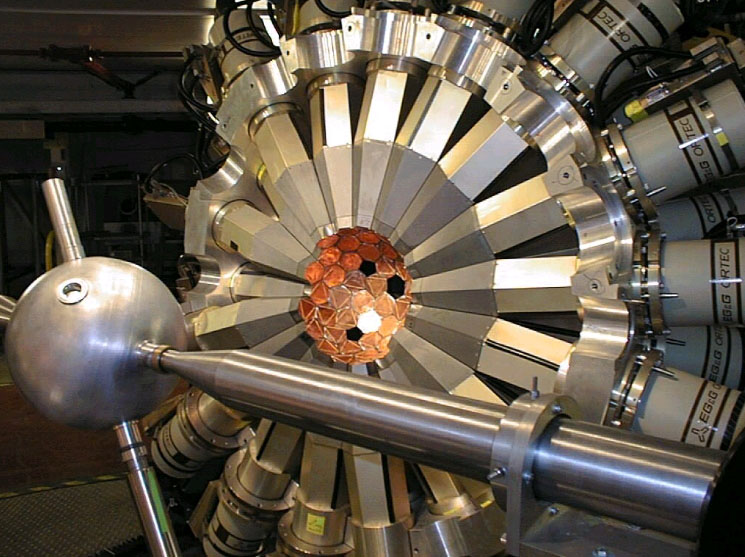
\includegraphics[height=0.3\textheight]{./img/c3/gammasphere_hemi.jpg}}
	\caption{View of scattering chamber and interior of one of Gammasphere's hemispheres drawn back from the chamber. The hexagonal copper foils are x-ray absorbers.}
	\label{fig:chp3-gs-hemisphere}
\end{figure}


\begin{figure}[h]
	\centerline{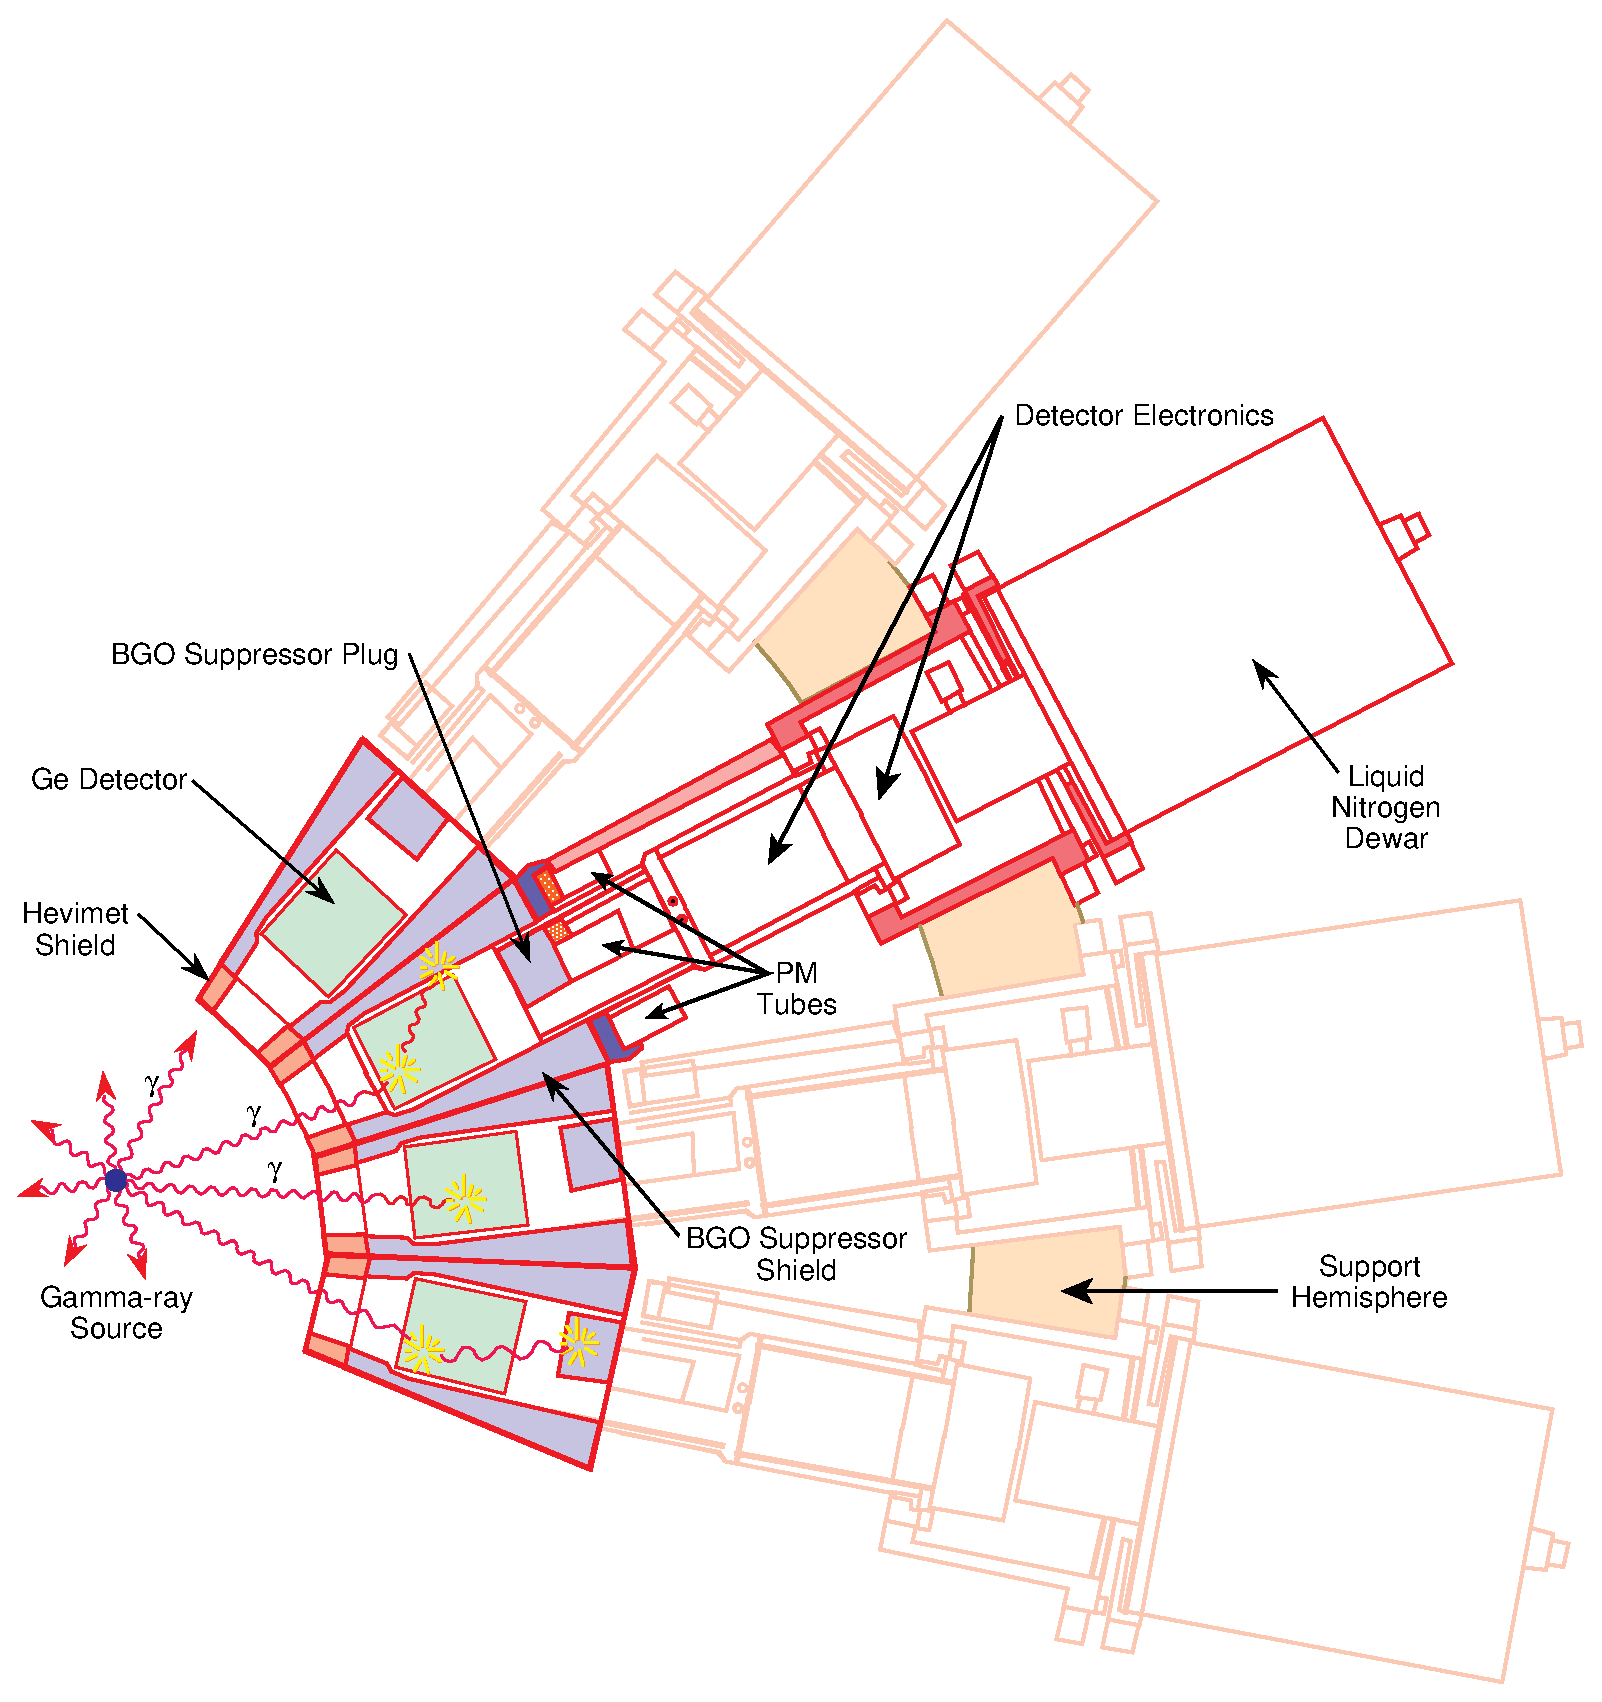
\includegraphics[height=0.3\textheight]{./img/c3/gammasphere_detector.eps}}
	\caption{Cross-section schematic of part of Gammasphere. Adapted from Ref.\cite{gsBooklet}}
	\label{fig:chp3-gs_det_schem}
\end{figure}


Honeycomb suppression is an escape suppression scheme that uses the BGO shields of adjacent detector modules to effectively double the thickness of a detector's shields. As seen in Fig. \ref{fig:chp3-gs_det_schem} almost every module will have additional modules immediately adjacent to it. If the HPGe detector for a given module do not register energy deposition the 6 side segments of its BGO shield are used to double the thickness of the shields they are adjacent to. Without this measure the singles P/T is $\sim0.62$; using honeycomb suppression improves this to $\sim0.69$ though it reduces the total efficiency at 1.332MeV from $\sim0.095$ to $\sim0.089$\cite{TheGS}. Table \ref{tbl:gs-summary} contains a brief summary of Gammasphere's features drawn from Refs. \cite{TheGS,SimulatedResGS,GSComptonSuppression,largeArrays}.

\begin{table}[h]
\caption{GAMMASPHERE FEATURE SUMMARY\label{tbl:gs-summary}}
\begin{center}
\begin{tabular}{|c|c|}
\hline
\hline No. Detectors             & 110 \\ 
No. Segmented Detectors   & 70 \\ 
HPGe Detector Size        & $7.1 cm$ (D) $\times$ $8.22 cm$ (L) \\
Detector Volume           & $312.8 cm^3$\\
Target to HPGe Front      & $24.6 cm$\\ 
Total HPGE Solid Angle    & $0.46 \times 4\pi$\\ 
Total Peak Efficiency     & $0.094$ at $1.3 MeV$\\ 
Singles P/T               & $0.6$ at $1.3 MeV$ \\ 
Energy Resolution (MeV)   & $2.1keV$ at $1.3 MeV$ \\ 
\hline 
\hline 
\end{tabular}
\end{center}
\end{table}

As mentioned in section \ref{ssec:exp-pr-gamma-spec-hpge} some of Gammasphere's detectors have a split outer electrode to reduce the effective half angle. Detector positions can be found in table \ref{tbl:app1-gs-rings} and table \ref{tbl:app1-gs-detectors} in appendix \ref{app:gs-rings-and-detectors}. Gammasphere's high granularity, good energy resolution, and efficiency make it a boon for high \gr{} multiplicity coincidence measurements.

\subsection{Indian National Gamma Array (INGA)}
\label{ssec:exp-pr-gamma-spec-inga}
The Indian National Gamma Array (pictured in Fig. \ref{fig:chp3-INGA}) is an array of 24 escape suppressed HPGe clover detectors\cite{ingaAtIUAC}. Since INGA utilizes clover detectors it is sensitive to the polarization of \gr{} emitted from nuclei in aligned states\cite{cloverDet}. Additionally, the use of clover detectors make the array more efficient for high energy \gr{} when using add back mode.

\begin{figure}[h!]
	\centerline{\includegraphics[height=0.25\textheight]{./img/c3/INGA.JPG}}
	\caption{Exterior view of INGA.}
	\label{fig:chp3-INGA}
\end{figure}

INGA's current incarnation utilizes a digital data acquisition system (DAQ) that allows it to run in a triggerless mode producing timestamped gamma data from a $10ns$ clock\cite{IngaDigitalDAQ}. Digital data acquisition systems, because they digitize the preamp signal directly, can operate at higher counting rates than analog because they do not require multiple microseconds of signal shaping time. The downside of this mode, is that coincidence are not prebuilt by the DAQ and instead need to be constructed by moving a sliding window of the desired coincidence time across the timeline of events and selecting sets of gammas that occur within that window. A final advantage of the time stamped events is that isomers can have their lifetime measured using time differences between \gr{}s as seen in Fig. \ref{fig:chp3-INGA-isomer}

\begin{figure}[h!]
	\centerline{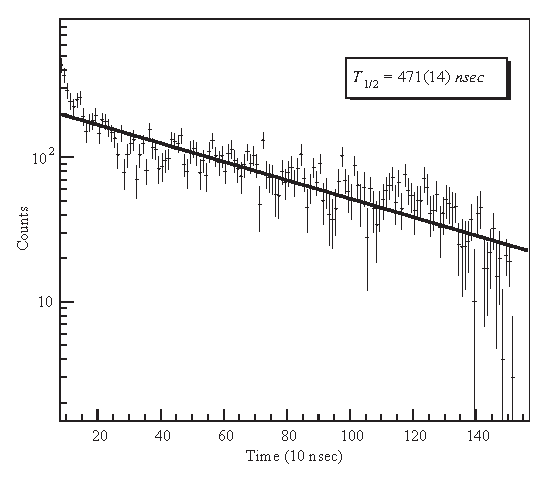
\includegraphics[height=0.35\textheight]{./img/c3/INGA_isomer.eps}}
	\caption{Example isomer timing spectrum for INGA. From Ref. \cite{IngaDigitalDAQ}.}
	\label{fig:chp3-INGA-isomer}
\end{figure}

Using its digital DAQ and add-back on the clover crystals, INGA achieves a total efficiency of $\sim0.05$ and P/T of $0.4$ at $\sim1.33MeV$. Table \ref{tbl:inga-summary} contains summary of INGA's features. INGA's sensitivity to polarization, efficiency, and granularity make it a good system for intermediate \gr{} multiplicity coincidence measurements, reaching its best efficiency at 2- to 3-fold events.

\begin{table}[h]
\caption{INGA FEATURE SUMMARY\label{tbl:inga-summary}}
\begin{center}
\begin{tabular}{|c|c|}
\hline
\hline
No. Clover Detectors      & 24\\ 
No. Single Crystals       & 96\\ 
Single Crystal Size       & $5 cm$ (D) $\times$ $7 cm$ (L) \\
Single Crystal Volume     & $117.5 cm^3$\\
Target to HPGe Front      & $24 cm$\\ 
Total HPGE Solid Angle    & $0.25 \times 4\pi$\\ 
Total Peak Efficiency     & $0.05$ at $\sim1.0 MeV$\\ 
Singles P/T               & $0.40$ at $1.3 MeV$ \\ 
Energy Resolution (MeV)   & $2.2keV$ at $1.3 MeV$ \\ 
\hline 
\hline 
\end{tabular}
\end{center}
\end{table}

\section{Experimental Details}
\label{sec:exp-pr-details}
The work on \pr{} presented in this dissertation was performed at two different facilities, the ATLAS (Argonne Tandem Linear Accelerator System) facility with the Gammasphere detector system, and the TIFR-BARC Pelletron LINAC with the INGA detector system. At both facilities the $^{16}O(^{123}Sb,4n)^{135}Pr$ reaction was used. As mentioned in section \ref{sec:exp-pr-fus-evap} the choice of beam and target affects both the most probable channel, the excitation energy, and the maximum angular momentum of the compound (and residual) nucleus. In previous in-beam \gr{} spectroscopy literature the following heavy ion fusion evaporation reactions have been used to reach yield the \pr{} residual nucleus: $^{120}Sn(^{19}F @ 91MeV,4n)^{135}Pr$\cite{Semkow135Pr}, $^{123}Sb(^{16}O @ 76MeV,4n)^{135}Pr$\cite{135PrLifetimes}, and  $^{116}Cd(^{23}Na @ 115MeV,4n)^{135}Pr$\cite{EPaul135Pr}. The $^{16}$O and $^{123}$Sb projectile-target combination was chosen for its lighter projectile to optimize for the population of states further from the yrast line.

\subsection{ATLAS/Gammasphere}
\label{ssec:exp-pr-details-gs}
ATLAS is located at the Physics Division at Argonne National Laboratory in Argonne, Illinois, USA. ATLAS is the world's first superconducting ac linear accelerator (linac) for projectiles heavier than an electron and consists of 3 sections. The first of these sections is the injector accelerator which can be either a 9 Megavolt (MV) tandem Van de Graff accellerator or an electron cyclotron resonance (ECR) ion source coupled to a 12 MV low velocity LINAC (PII, Positive Ion Injector). The beam from the chosen injector is sent the 20 MV ``booster'' linac and finally to the 20 MV ``ATLAS'' linac. This system produces pulsed beams with spot diameter $\leq1mm$, pulse length $\leq500ps$, and interval $82ns$ which range across all elements from hydrogen to uranium with energies of $7-17MeV$ per nucleon ($/\mu{}$.)

The Gammasphere detector system was used in the FMA (Fragment Mass Analyzer) position though the FMA itself was not used. This configuration requires that the first ring of detectors at $\theta{}=17.27465^{\circ}$ be removed from the array due to a lack of space. Additionally there were several other detectors removed from the array due to various issues. A complete listing of the detector numbers missing from the array is presented in Table \ref{tbl:app1-gs-missing-det} in Appendix \ref{app:gs-rings-and-detectors}.

Multiple self supporting $^{123}$Sb targets were prepared for the experiment using 98.28\% enriched powder from ISOFLEX USA (PO Box 29475, San Francisco, CA 94129 USA)\cite{sbTargets}. Due to the low thermal conductivity ($0.243W/cm/K$ at $300K$\cite{thermalCond}) and high vapor pressure\cite{sbPartialP,sbTargets} of Sb a thin layer ($14\mu{}g/cm^2$) of Al was deposited on the front surface of several of the targets created. This served the dual purpose of helping to dissipate the heat deposited in the target by the beam and of inhibiting sputtering of the target. Of the targets that had the Al layer, two ($630\mu{}g/cm^2$ and $634\mu{}g/cm^2$) were placed on the target ladder for Gammasphere (as well as a beam viewer). An oxygen beam of $3pnA$ at $81.2MeV$ was then impinged on the $634\mu{}g/cm^2$ target (the other target served as an unnecessary backup in case of failure of the primary target.) To further reduce the risk of evaporating a hole in the target, the beam was wobbled by $\pm{}3mm$. \emph{Note to self: Get the correct values for wobbling distance and beam current from logbook to replace these approximate values}

\subsection{TIFR - BARC Pelletron LINAC / INGA}
\label{ssec:exp-pr-details-inga}
The TIFR-BARC pelletron linac is located at the Tata Institute of Fundamental Research (TIFR), Mumbai, India. It is a collaborative project between TIFR and the Bhabha Atomic Research Centre (BARC) and is the first superconducting heavy ion accelerator in India. The first section of the system is a 14MV tandem Van de Graaf accelerator. The beam emitted from the pelletron is then bunched and injected into a linac yielding beam pulses with a width of $\sim{}600ps$ ranging across most of the elements from hydrogen to chlorine at $5-10MeV/\mu{}$.

The INGA detector system was used in its standard position at the facility, however a few detectors were not present due to various problems. A summary of the electronics connections and which detectors were and were not present is in Table \ref{tbl:app2-inga-detectors}. Two of the pockets of INGA had Ce activated LaBr$_3$ detectors though they were not used. \emph{Note to self: Get the pocket numbers from the logbook}.

The two self supporting targets used in the Gammasphere experiment were given a thick gold backings of $20.3mg/cm^2$ for the $630\mu{}g/cm^2$ target and $22.8mg/cm^2$ for the $634\mu{}g/cm^2$\cite{sbTargets}. This served several purposes: First and foremost the thick backing helped the delicate Sb targets survive transport to India. Second, there was hope it would be possible to extract lifetimes for transverse wobbling states (this unfortunately proved impossible.) Finally, the thick gold backing allowed heat deposited in the target by the beam to be easily dissipated, negating the need for a beam wobbling system.

\section{Data Processing}
\label{sec:exp-pr-data-proc}
 As stated earlier, this work was performed at two different facilities. In the experiment using Gammasphere $\sim{}185$Gb of data spread across $104$ files were collected. This data was comprised of $3.57\times{}10^9$ three- and higher-fold events with the distribution across folds shown in Fig. \ref{fig:chp3-gs_event_pattern}. While the system was set to not trigger for less than three-fold events, lower events still make it through due to honeycomb suppression. Because, honeycomb suppression is applied after the system has triggered it effectively remove gammas from an event, reducing its fold, even to below the threshold set in the trigger system. The data from this experiment was used for the reconstruction of the level scheme and extraction of angular distributions and DCO Ratios.
 
\begin{figure}[h!]
	\centerline{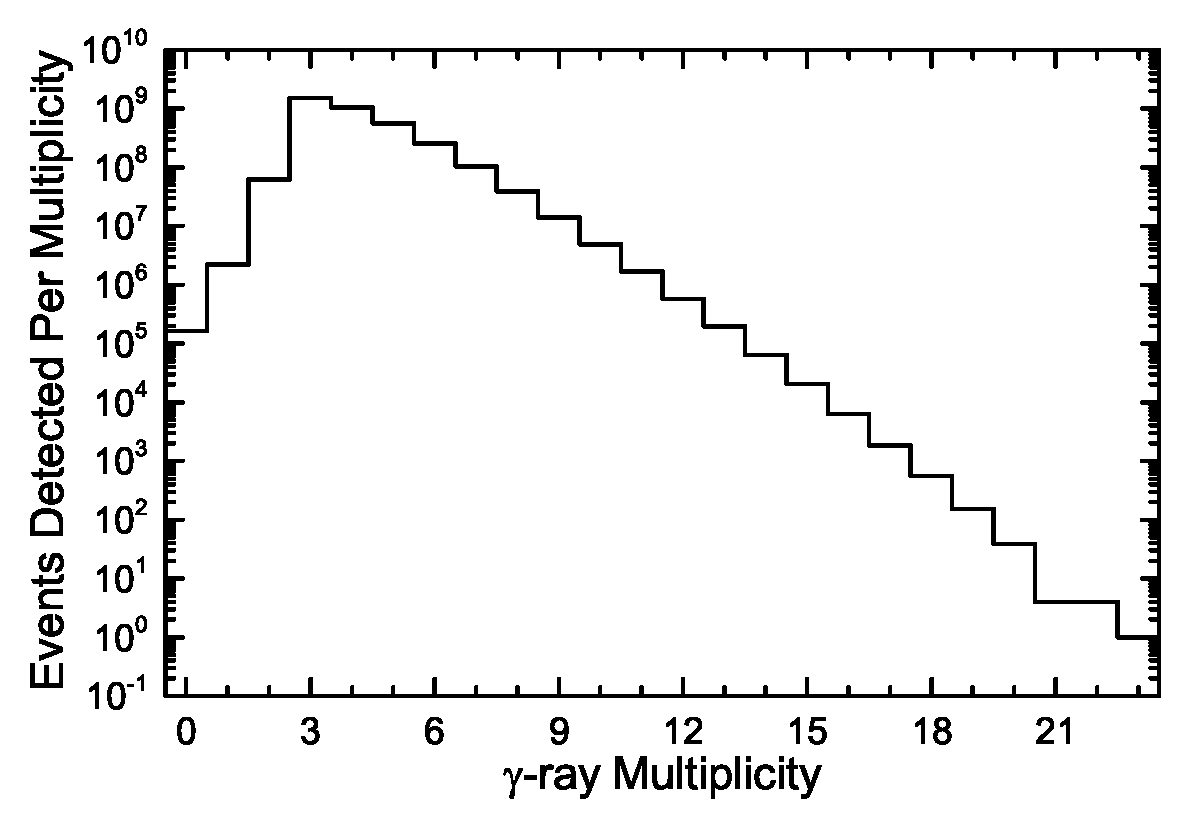
\includegraphics[height=0.25\textheight]{./img/c3/gs_event_plot.eps}}
	\caption{Histogram of the number of events in each multiplicity for the experiment at Gammasphere.}
	\label{fig:chp3-gs_event_pattern}
\end{figure}
 
 In the experiment utilizing INGA $\sim{}550$Gb of data spread across $\sim800$ files were collected. As INGA was run in a triggerless mode each module of electronics output timestamped events in each detector to a file. Afterwards the data are merged into an order according to their timestamp, yielding $\sim{}503$Gb spread across $185$ files. Construction of events then proceeds by setting a coincidence time window and ``scanning'' the window across the merged events looking for sets of events whose timestamps all fall within that window. This process yielded $3.52\times{}10^9$ two- and higher-fold events. This data was used for the extraction of polarizations using the scattering asymmetry at $90^{\circ{}}$. This, coupled with requiring that the energy be seen in two and \emph{only} two of the crystals of a $90^{\circ{}}$ detector, reduced the number of eligible two- and higher-fold events to $3.47\times{}10^8$.
 
\subsection{Calibration}
\label{ssec:exp-pr-data-proc-cal}
Prior to working with the actual data in an experiment it is necessary to perform energy and efficiency calibration of the detectors. For \gr{} detection experiments of this kind calibration involves placing a radioactive source with known lines in the same position that the beam would strike the target. If absolute efficiency is desired as opposed to relative efficiency the activity of the source must be known as well so that one know exactly how many gamma's passed through one's detector. In this case however, only relative efficiency was necessary so this information was neglected.

At the Gammasphere experiment a $^{152}$Eu source was used for calibration. $^{152}$Eu has many peaks but the $10$ strongest (non-overlapping) peaks were chosen for use. An example spectrum from a typical detector with the chosen peaks numbered can be found in Fig. \ref{fig:chp3-gs-cal-spec}.  A table of the energies and relative intensities of these peaks can be found in table \ref{tbl:152Eu-peaks}. For the INGA experiment a $^{152}$Eu and $^{133}$Ba mixed source was used for calibration purposes, a listing of the energies and relative intensities of the $^{133}$Ba peaks can be found in table \ref{tbl:133Ba-peaks}. An example of a single crystal spectrum for INGA can be found in \ref{fig:chp3-inga-cal-spec}. Here because the peaks are due to both $^{152}$Eu and $^{133}$Ba they are labeled with both the index number of the peak and a superscript denoting which nuclide was their origin.

\begin{figure}[h!]
	\centerline{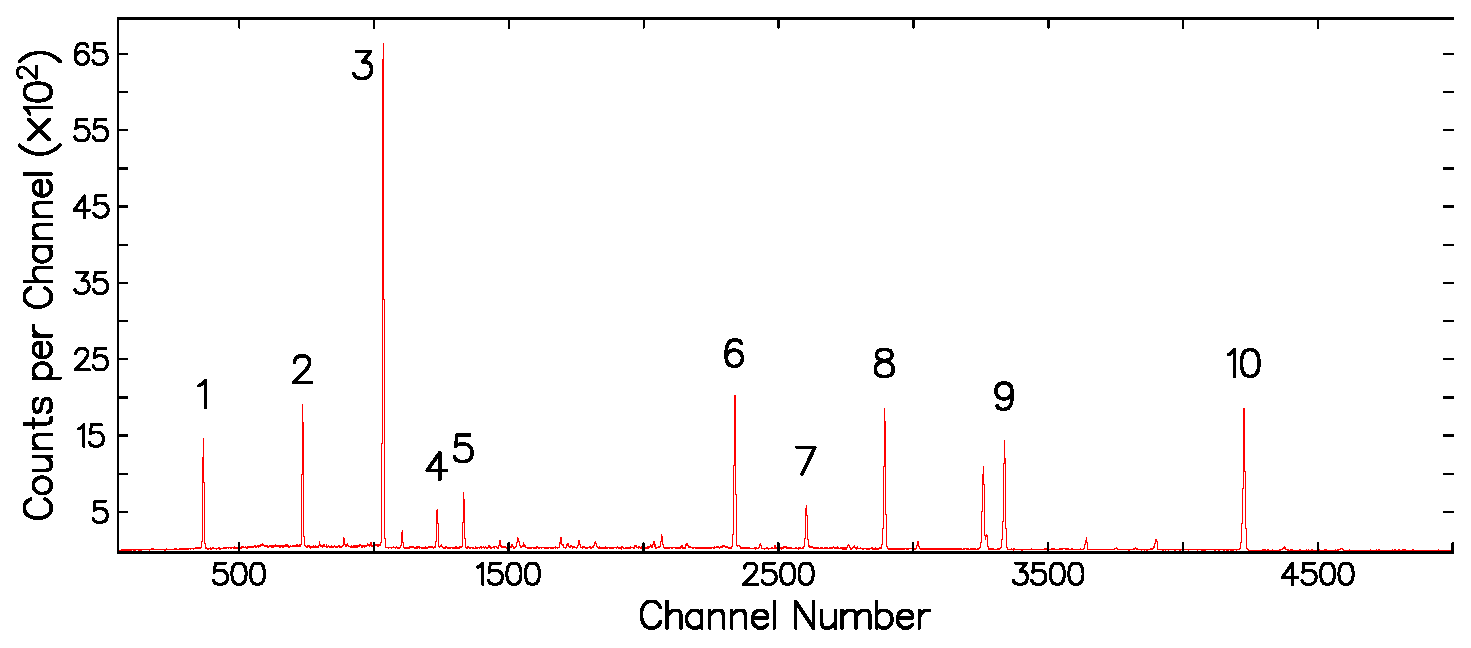
\includegraphics[height=0.25\textheight]{./img/c3/gs_cal_spec.eps}}
	\caption{$^{152}$Eu calibration spectrum from a typical Gammasphere detector.}
	\label{fig:chp3-gs-cal-spec}
\end{figure}

\begin{table}
\caption{$^{152}$Eu PEAK DATA \label{tbl:152Eu-peaks}}
\begin{center}
\begin{tabular}{ccc}
\toprule
Peak No. & Energy (keV) & Rel. Intensity. \\ 
\midrule
1 & $121.783(2)$ & $13620(160)$ \\ 
2 & $244.692(2)$ & $3590(60)$ \\ 
3 & $344.276(4)$ & $12750(90)$ \\ 
4 & $411.115(5)$ & $1070(10)$ \\ 
5 & $443.976(5)$ & $1480(20)$ \\ 
6 & $778.903(6)$ & $6190(80)$ \\ 
7 & $867.388(8)$ & $1990(40)$ \\ 
8 & $964.131(9)$ & $6920(90)$ \\ 
9 & $1112.116(17)$ & $6490(90)$ \\ 
10 & $1408.011(14)$ & $10000(30)$ \\ 
\bottomrule
\end{tabular} 
\end{center}
\end{table}

\begin{table}
\caption{$^{133}$Ba PEAK DATA \label{tbl:133Ba-peaks}}
\begin{center}
\begin{tabular}{ccc}
\toprule
Peak No. & Energy (keV) & Rel. Intensity. \\ 
\midrule
1 & $80.999(4)$ & $5120(40)$ \\ 
2 & $276.404(7)$ & $1130(10)$ \\ 
3 & $302.858(5)$ & $2920(30)$ \\ 
4 & $356.014(9)$ & $10000(30)$ \\ 
5 & $383.859(9)$ & $1450(20)$ \\ 
\bottomrule
\end{tabular} 
\end{center}
\end{table}
\begin{figure}[h!]
	\centerline{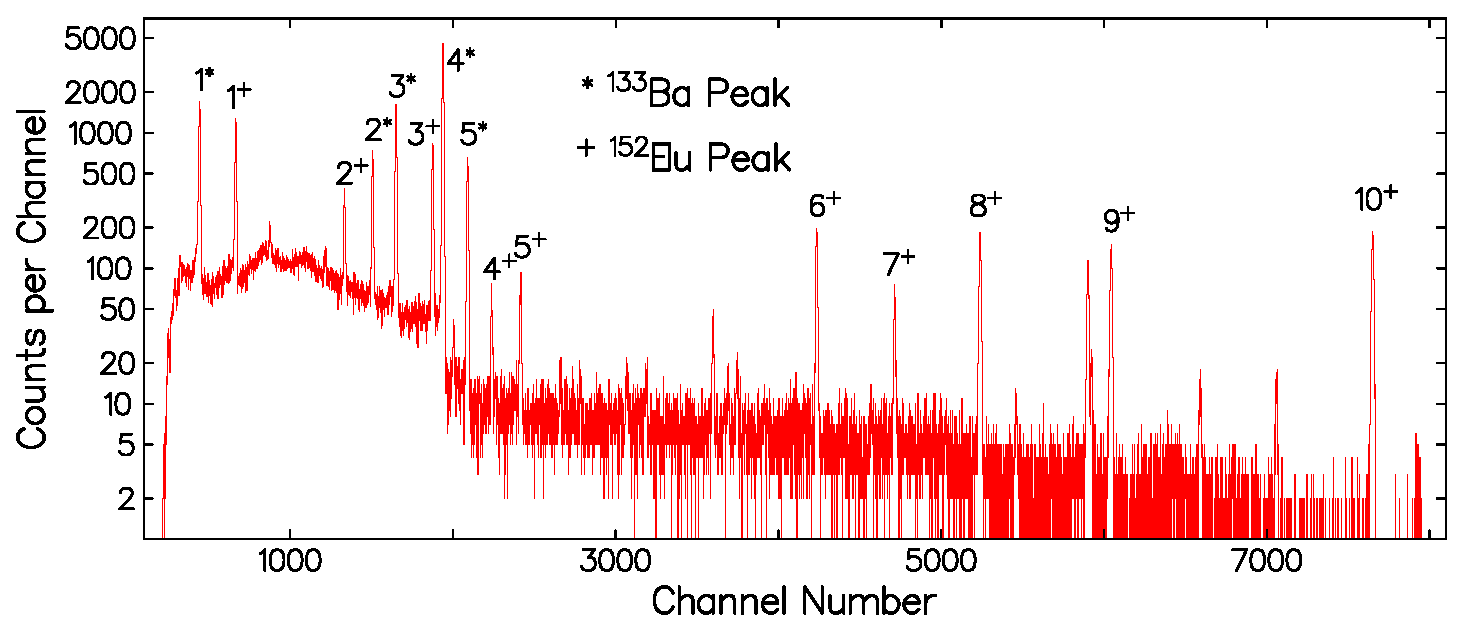
\includegraphics[height=0.25\textheight]{./img/c3/inga_crystal_en_cal.eps}}
	\caption{Typical $^{152}$Eu and $^{133}$Ba mixed source calibration spectrum from a single crystal of an INGA clover detector.}
	\label{fig:chp3-inga-cal-spec}
\end{figure}
For Gammasphere, after extraction of the spectra, energy calibration of each detector proceeded as follows. First, using the program \emph{gf3} from the Radware tool suite\cite{radware}, each of the $10$ peaks was fit with a gaussian peak shape plus linear background whose formula is:
\begin{equation}
\label{eqn:pk_fit} 
Fit(x) = h\exp{}^{-\frac{(x-\mu{})^2}{2\sigma{}^2}} + a + b (x-\overline{x})
\end{equation}
 Where $h$ is the peak height, $\mu{}$ is the peak centroid, $2\sqrt{2ln(2)}\sigma{}$ is the FWHM of the peak, $a$ is the constant term of the background, $b$ is the linear term of the background, and $\overline{x}$ is the center of the region to be fitted. From these fits the peak area ($\sqrt{2\pi{}}\sigma{}h$) and centroid are extracted. For energy calibration the centroids are then combined with the corresponding energies and are fit with polynomials (as in eqn \ref{eqn:en_cal}) from $2^{nd}$ to $5^{th}$ order.

\begin{equation}
\label{eqn:en_cal} 
E = a_0 + a_1x + a_2x^2 + a_3x^3 + a_4x^4 + a_5x^5
\end{equation}

After this the reduced $\chi{}^2$ of the fits ($\chi^2/d.o.f.$) were compared and the polynomial with the lowest reduced $\chi{}^2$ was selected to be the energy calibration for that detector. A listing of the energy calibration parameters used for Gammasphere can be found in table \ref{tbl:app1-gs-en-cal}.

For INGA, following the extraction of single crystal spectra, energy calibration was performed by using \emph{gf3} to fit each of the peaks of interest to extract the positions of each peak. After gathering the peak positions and combining them with their respective energies a $2^{nd}$ order polynomial was fit. No higher order polynomials were used due to both the enhanced linearity of a digital data acquisition system and limitations in the code used for further analysis. A listing of the energy calibration parameters used for INGA can be found in table \ref{tbl:app2-inga-en-cal}.

For Gammasphere the peak areas were divided by the corresponding relative intensities in table \ref{tbl:152Eu-peaks} to give the relative efficiency of each peak, following energy calibration. Then, using the program \emph{effit} from the Radware suite, the energies and relative efficiencies of each peak were then fitted with:
\begin{equation}
\label{eqn:eff_cal} 
ln(\epsilon) = [(A+Bx+Cx^2)^{-G} + (D+Ey+Fy^2)^{-G}]^{-1/G}
\end{equation}
Here $A$, $B$, $C$ are parameters that control the low energy part of the efficiency, though $C$ is usually set to $0.0$. $D$, $E$, $F$ are the parameters that control the high energy component of the efficiency. $G$ is the parameter that controls the ``sharpness'' of the intermediate energy turnover region where they play equal roles. The parameters $x$ and $y$ are related to the \gr{} energy as follows:
\begin{align*}
\label{eqn:eff_x_and_y}
x=ln(\frac{E_{\gamma{}}}{100~keV}) && y=ln(\frac{E_{\gamma{}}}{1000~keV})
\end{align*}
A plot of extracted relative efficiencies and the fit to them for a Gammasphere detector can be found in Fig. \ref{fig:chp3-gs-eff_plot}. A listing of the relative efficiency calibration parameters used for Gammasphere can be found in table \ref{tbl:app1-gs-en-cal}.

\begin{figure}[h!]
	\centerline{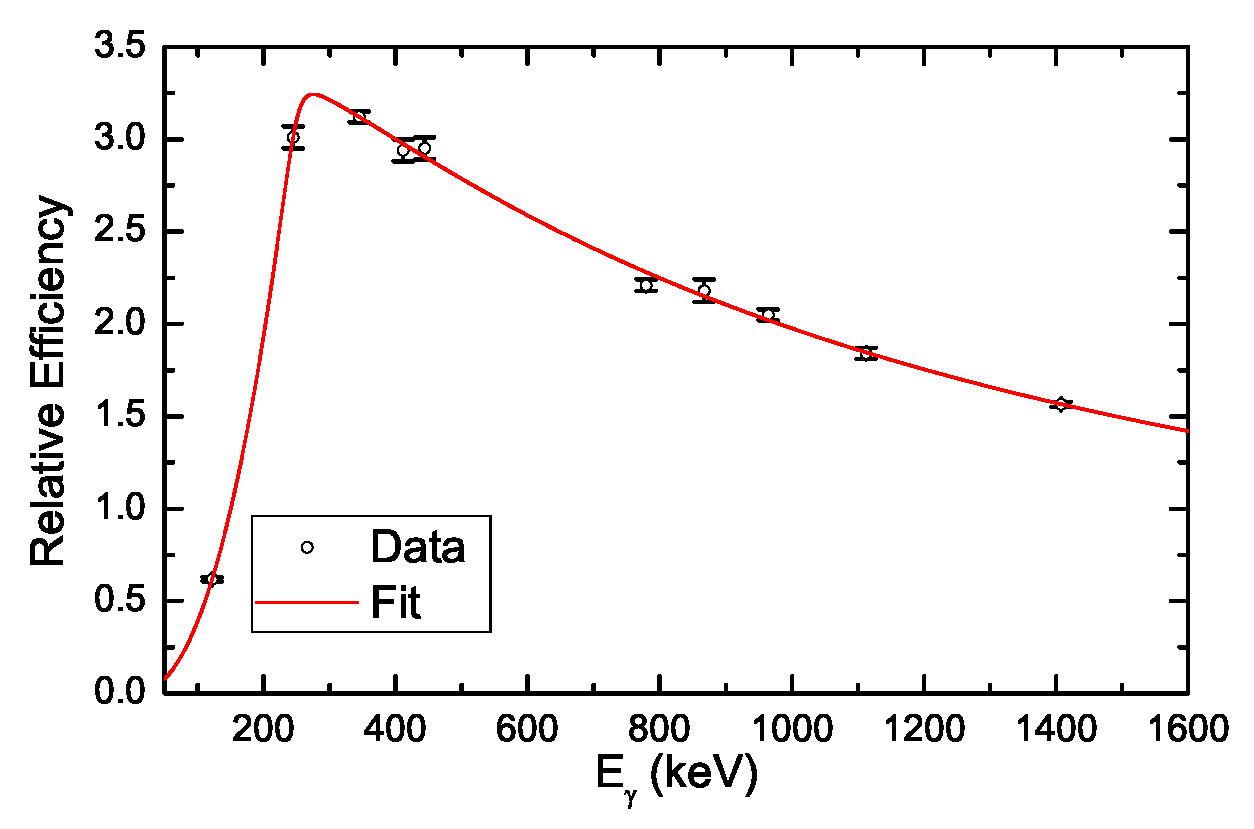
\includegraphics[width=0.9\textwidth]{./img/c3/gs_eff_plot.eps}}
	\caption{$^{152}$Eu extracted relative efficiencies and fit.}
	\label{fig:chp3-gs-eff_plot}
\end{figure}

As it was unnecessary for the asymmetry analysis performed on the INGA data a relative efficiency calibration was not performed. If one had been necessary one would need to know the ratio of the $^{133}$Ba and $^{152}$Eu source activities or include that ratio as an eighth parameter of the fit. This would allow one to normalize the relative efficiencies of the peaks from the two sources to the same scale.

\subsection{Level Scheme Scheme Determination}
\label{ssec:exp-pr-data-proc-lvl-scheme}

\subsection{Background Subtraction}
\label{ssec:exp-pr-data-proc-bg-sub}
Any time one places a gate on \gr{} they need to account for background counts.
\subsubsection{Symmetric Gates}
\label{sssec:exp-pr-data-proc-bg-sub-sym}
\subsubsection{Asymmetric Gates}
\label{sssec:exp-pr-data-proc-bg-sub-asym}

\section{Angular Distributions, Correlations, and Polarization}
\label{sec:exp-pr-data-ang}
\subsection{Angular Distributions}
\label{ssec:exp-pr-data-ang-dist}
Testing 1
\subsection{Angular Correlations}
\label{ssec:exp-pr-data-ang-cor}
\begin{figure}[h!]
	\centerline{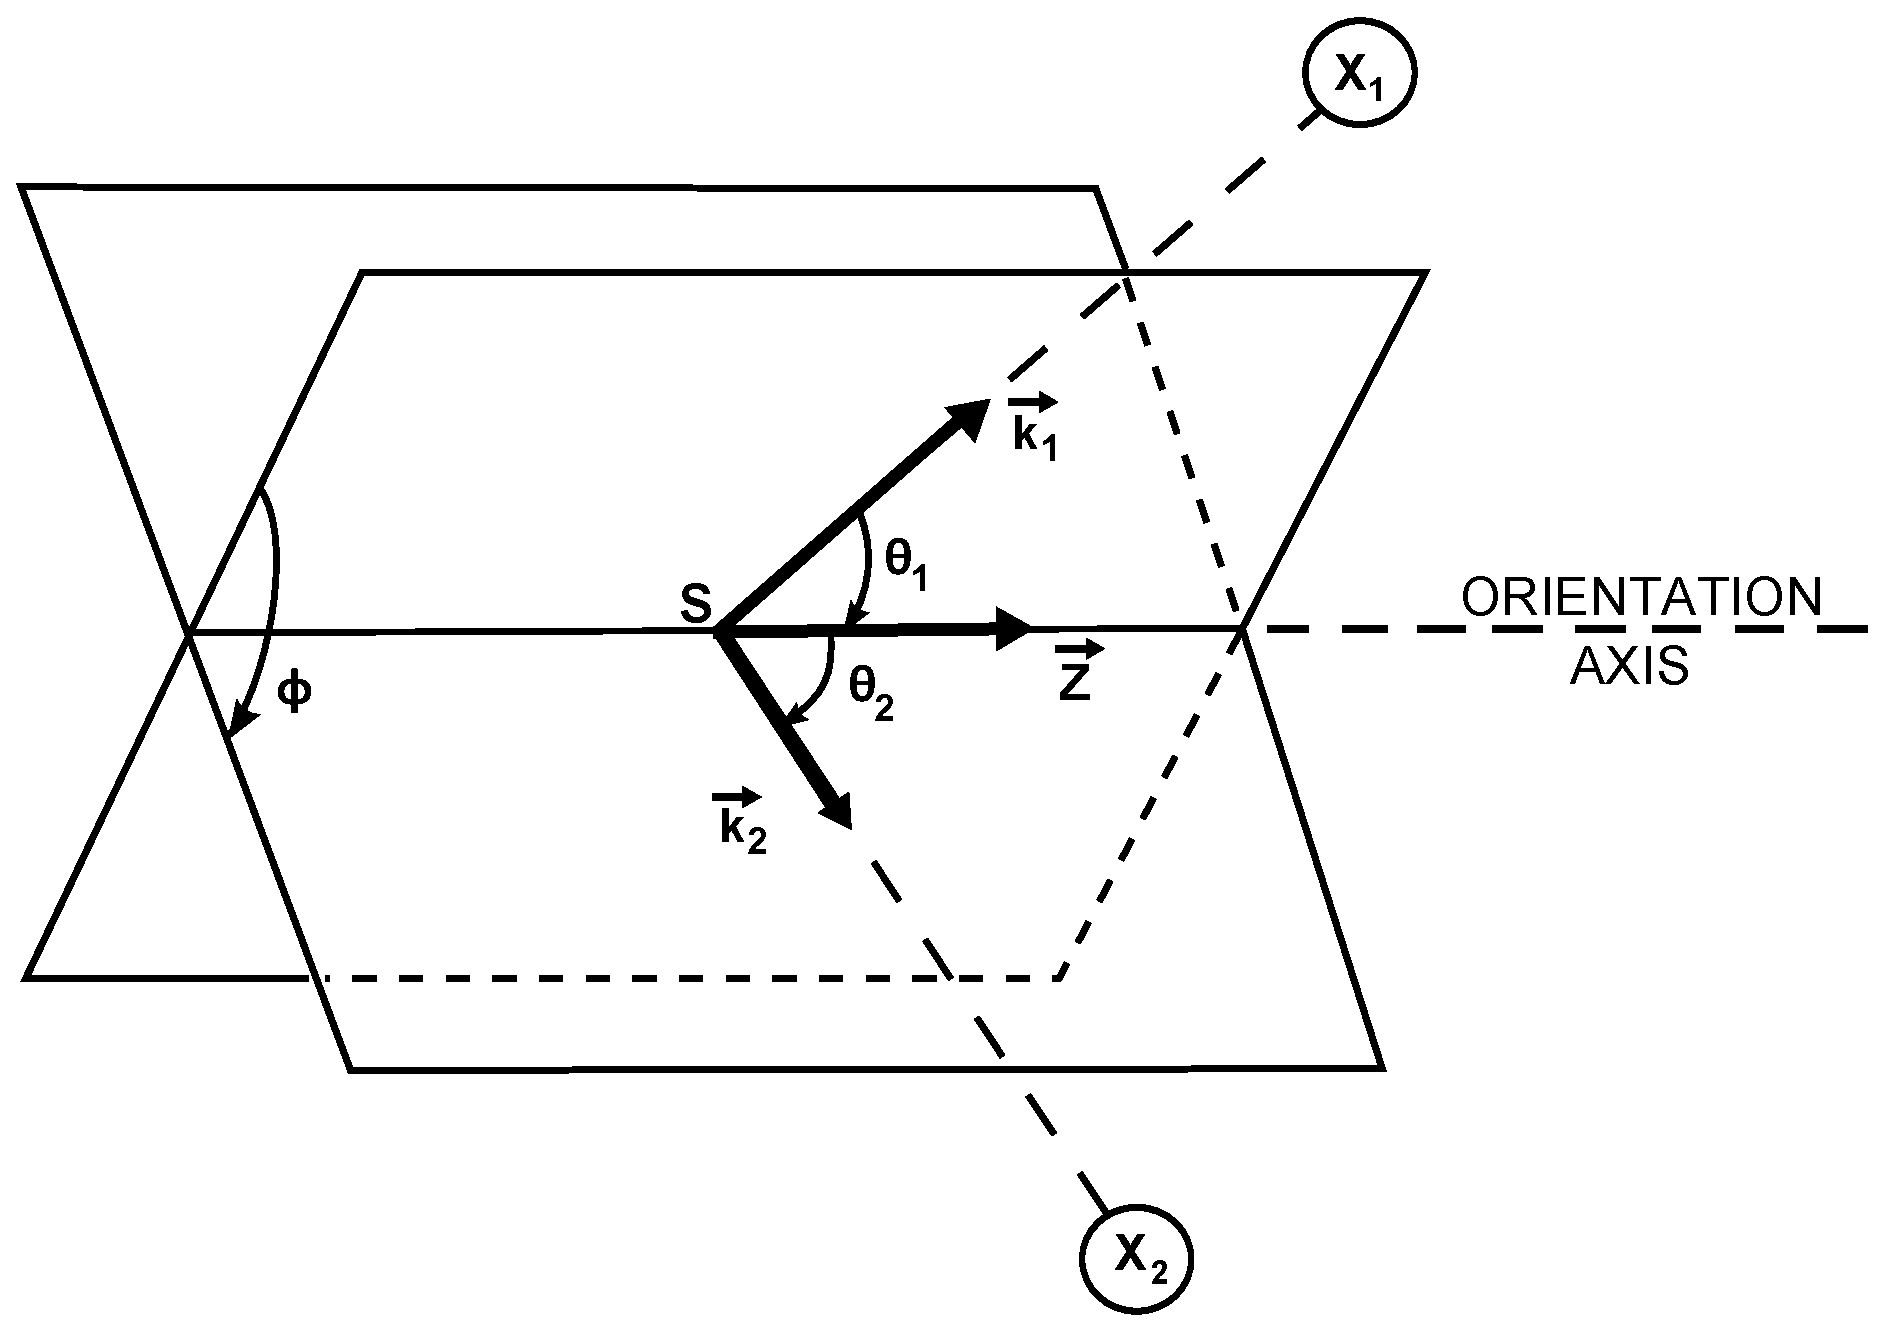
\includegraphics[height=0.35\textheight]{./img/c3/dco_setup.eps}}
	\caption{Diagram of the angles in a directional correlation of two successive radiations X$_{1}$ and X$_{2}$ emitted from an axial symmetric oriented source S.}
	\label{fig:chp3-DCO-Angles}
\end{figure}
\subsubsection{Directional Correlation of Gamma-rays from Oriented Nuclei DCO Ratios}
\label{sssec:exp-pr-data-ang-cor-dco}
Testing 3
\subsection{Polarization}
\label{ssec:exp-pr-data-ang-pol}
Testing 4
